\documentclass{article}

\usepackage{circuitikz}
\usepackage[T1]{fontenc} 
\usepackage[UTF8]{inputenc}
\usepackage{amsmath}
\usepackage{amssymb}
\usepackage{fancyhdr}
\usepackage{graphicx}
\usepackage{hyperref}
\usepackage{tikz}
  \usetikzlibrary{arrows}
  \usetikzlibrary{shapes}
  \usetikzlibrary{arrows.meta,topaths}
  \usetikzlibrary{bending}
  \usetikzlibrary{calc}
\usepackage{anyfontsize}
\usepackage{sectsty}
\usepackage{../assets/scripts/tex/color-env}
\usepackage{anyfontsize}
\usepackage{xcolor}
\definecolor{DarkGreenBlue}{HTML}{264653}
\definecolor{LightGreenBlue}{HTML}{2A9D8F}
\definecolor{LightOrange}{HTML}{E9C46A}
\definecolor{DarkOrange}{HTML}{F4A261}
\definecolor{RedOrange}{HTML}{E76F51}
\definecolor{BrightRed}{HTML}{D62828}
\definecolor{DeepBlue}{HTML}{003049}



\usepackage[ngerman]{babel}
\title{Elektrotechnik 1 - Praktikum 3}


\usepackage[
  includehead,
  headheight = 17mm,
  footskip = \dimexpr\headsep+\ht\strutbox\relax,
  tmargin = 0mm,
  bmargin = \dimexpr17mm+2\ht\strutbox\relax,
]{geometry}





\pagestyle{fancy}
\fancyhead[L]{\leftmark}
\fancyhead[R]{}
\fancyfoot[L]{}
\fancyfoot[C]{\thepage}
\fancyfoot[R]{
\includegraphics[scale=0.2]{../assets/images/haw.jpg}}
\renewcommand\headrulewidth{0.5pt}


\begin{document}


\thispagestyle{empty}
\begin{tikzpicture}[remember picture,overlay]

  \fill[DeepBlue] (current page.south west) rectangle (current page.north east);

  \begin{scope}

    \foreach \i in {2.5,...,22}
      {
        \node[rounded corners, DeepBlue!90,draw ,regular polygon, regular polygon sides=6, minimum size=\i cm, ultra thick] at ($(current page.west)+(2.5,-5)$) {} ;
      }

  \end{scope}

  \node[rounded corners,fill=DeepBlue!95,text =DeepBlue!5,regular polygon,regular polygon sides=6, minimum size=2.5 cm,inner sep=0,ultra thick] at ($(current page.west)+(2.5,-5)$) {\LARGE \bfseries 2020};

  \foreach \i in {0.5,...,22}
    {
      \node[rounded corners,DeepBlue!90,draw,regular polygon,regular polygon sides=6, minimum size=\i cm,ultra thick] at ($(current page.north west)+(2.5,0)$) {} ;
    }

  \foreach \i in {0.5,...,22}
    {
      \node[rounded corners,DeepBlue!98,draw,regular polygon,regular polygon sides=6, minimum size=\i cm,ultra thick] at ($(current page.north east)+(0,-9.5)$) {} ;
    }

  \foreach \i in {12}
    {
      \node[fill = DeepBlue,rounded corners,draw=DeepBlue,regular polygon,regular polygon sides=6, minimum size=\i cm,ultra thick] at ($(current page.south east)+(-0.2,-0.45)$) {} ;
    }


  \foreach \i in {21,...,6}
    {
      \node[DeepBlue!95,rounded corners,draw,regular polygon,regular polygon sides=6, minimum size=\i cm,ultra thick] at ($(current page.south east)+(-0.2,-0.45)$) {} ;
    }

  \node[left,DeepBlue!5,minimum width=0.625*\paperwidth,minimum height=3cm, rounded corners] at ($(current page.north east)+(0,-9.5)$){{\fontsize{25}{30} \selectfont \bfseries ET2 - Praktikum 5}};

  \node[left,DeepBlue!10,minimum width=0.625*\paperwidth,minimum height=2cm, rounded corners] at ($(current page.north east)+(0,-11)$){{\huge \textit{Resonanz}}};

  \node[left,DeepBlue!5,minimum width=0.625*\paperwidth,minimum height=2cm, rounded corners] at ($(current page.north east)+(0,-13)$){{\Large \textsc{Florian Tietjen\hspace{0.5cm}Eric Antosch}}};

\end{tikzpicture}

\newpage
\thispagestyle{empty}

\tableofcontents


\newpage


\section{Vorbereitung}
Als Vorbereitung der folgenden Versuche werden vorher einige Kenngrößen eines Serienresonanzkreies berechnet.
Die Serienschaltung besteht dabei aus einer Induktivität L = 100 mH und einem Gleichstrom-Drahtwiderstand $R_L = 10 \Omega$ . Der Sinus-Generator
hat einen Innenwiderstand von $R_i = 50\Omega$. Die angegebene Größe der Induktivität gilt nur für Frequenzen f < 1kHz.

\subsection{Berechnung der erforderlichen Kapazität}
Die Formel zur Berechnung der Resonanzfrequenz wird nach der Kapazität C umgestellt.
\begin{align*}
  \omega_r & = \frac{1}{\sqrt{LC}} \\
  C        & = \frac{1}{{w_r}^2L}
\end{align*}
Mit der Formel werden nun die Kapazitäten verschiedener Frequenzen ausgerechnet:
\begin{table}[h]
  \begin{center}
    \begin{tabular}{|c|c|c|c|c|c|}
      \hline
      Frequenz  & $100 Hz$     & $500Hz$      & $1kHz$    & $5kHz$    & $10kHz$  \\
      \hline
      Kapazität & $25,33\mu F$ & $1,013\mu F$ & $253,3nF$ & $10,13nF$ & $2,53nF$ \\
      \hline
    \end{tabular}

  \end{center}
\end{table}

\subsection{Berechnung der Gütefaktoren und Bandbreiten}
Nun werden die zugehörigen Gütefaktoren Q und Bandbreiten $\Delta$f für jeweils den Gesamtverlustwiderstand R$_i$ + R$_L$ und den Spulen-Drahtwiderstand R$_L$ allein berechnet.
Für den Gesamtverlustwiderstand gilt:
\begin{align*}
  R_{ges} & = R_i + R_L= 50\Omega + 10\Omega = 60\Omega
\end{align*}
Die Formel der Güte einer Serienschaltung lautet:
\begin{align*}
  Q & = \frac{1}{R}\cdot\sqrt{\frac{L}{C}}
\end{align*}
Für die Bandbreite $\Delta$f ermittelt sich aus:
\begin{align*}
  B & = \frac{f_r}{Q}
\end{align*}
Für verschiedene Frequenzen ergeben sich dann folgende Güten und Bandbreiten:
\begin{table}[h]

  \begin{center}

    \begin{tabular}{|c|c|c|c|c|c|}
      \hline
      Frequenz             & $100Hz$ & $500Hz$ & $1kHz$  & $5kHz$   & $10kHz$  \\
      \hline
      $Q_{R_{ges}}$        & $1,05$  & $5,24$  & $10,47$ & $52,37$  & $104,78$ \\
      \hline
      $Q_L$                & $6,28$  & $31,42$ & $62,83$ & $316,02$ & $628,7$  \\
      \hline
      $\Delta f_{R_{ges}}$ & $95,24$ & $95,42$ & $95,51$ & $95,47$  & $95,44$  \\
      \hline
      $\Delta f_L$         & $15,92$ & $15,91$ & $15,92$ & $15,82$  & $15,91$  \\
      \hline
    \end{tabular}
    \caption{Güte und Bandbreite in Abhängigkeit von dem betrachtetem Widerstand und der Frequenz}
    \label{tab:cGB}
  \end{center}
\end{table}
s



\newpage

\section{Resonanz - Eingeschwungener Zustand}
\begin{devlist}
  T
  \begin{itemize}
    \item Oszilloskop: Tektronix MDO3012
    \item Funktionsgenerator: Rhode und Schwarz HM 8150
    \item Operationsverstärker-Impedanzwandler HPS 9240
    \item Multimeter: MetraHit TECH Multimeter
  \end{itemize}
\end{devlist}
\subsection{Versuch 1}
\begin{task}
  IIm ersten Versuch soll der Amplitudengang von $\hat{u}_C$ in der abgebildeten Schaltung mit dem Oszilloskop ermittelt werden. Dazu soll beachtet werden,
  dass $R_i = 50\Omega$ und $\hat{u}_{gen} = 1V$ sind. Die Kapazitätsdekade wird mit den berechneten Werten aus der Vorbereitung eingestellt.
\end{task}


\begin{figure}[h!]
  \begin{center}
    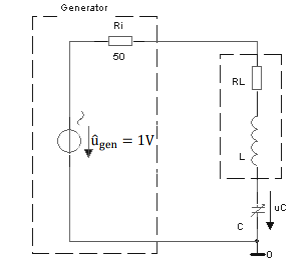
\includegraphics{../assets/images/ETP3/Versuch1Schaltplan.PNG}
    \caption{Schaltplan zum ersten Versuch der ersten Aufgaben zur Bestimmung des Spannungsverhältnisses $\frac{\hat{u}_C}{\hat{u}_{gen}}$}
  \end{center}
\end{figure}

\newpage

\subsubsection{Bestimmung von $\frac{\hat{u}_C}{\hat{u}_{gen}}$}

\begin{table}[h]
  \begin{center}

    \begin{tabular}{|c|c|c|}
      \hline
      $\Delta$f & $f_r = 500Hz, C=1,01\mu F$ & $f_r = 1kHz, C= 253,3 nF$ \\
      \hline
      -95       & 2,64V                      & 5,2V                      \\
      \hline
      -50       & 4V                         & 8V                        \\
      \hline
      -40       & 4,4V                       & 8,8V                      \\
      \hline
      -20       & 5,04V                      & 10V                       \\
      \hline
      -10       & 5,12V                      & 10,2V                     \\
      \hline
      -5        & 5,12V                      & 10,2V                     \\
      \hline
      0         & 5,04V                      & 10V                       \\
      \hline
      5         & 5,12V                      & 9,6V                      \\
      \hline
      10        & 4,8V                       & 9,4V                      \\
      \hline
      20        & 4,4V                       & 8,6V                      \\
      \hline
      40        & 3,6V                       & 7V                        \\
      \hline
      50        & 3,2V                       & 6,4V                      \\
      \hline
      95        & 2V                         & 4,2V                      \\
      \hline
    \end{tabular}
    \caption{Messwerte für Versuch 1.1}
    \label{tab:MV}
  \end{center}
\end{table}


\newpage

\subsubsection{Graphische Darstellung der Ergebnisse}
\begin{figure}[h]
  \begin{center}
    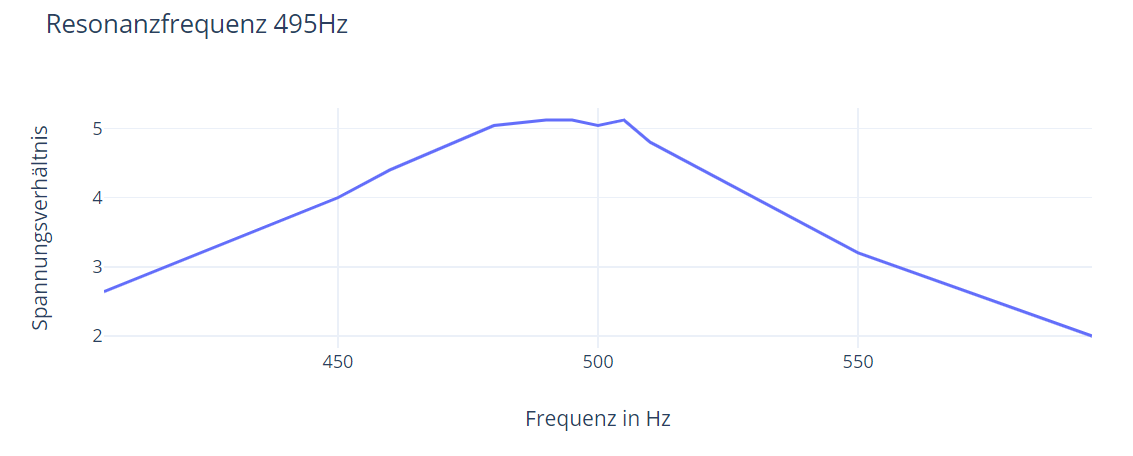
\includegraphics[scale=0.75]{../assets/images/ETP3/Fre495Plot1.PNG}
    \caption{Darstellung des Spannungsverhältnisses in Abhängigkeit der Frequenz ($f_r = 495Hz$)}
  \end{center}
\end{figure}

\begin{figure}[h]
  \begin{center}
    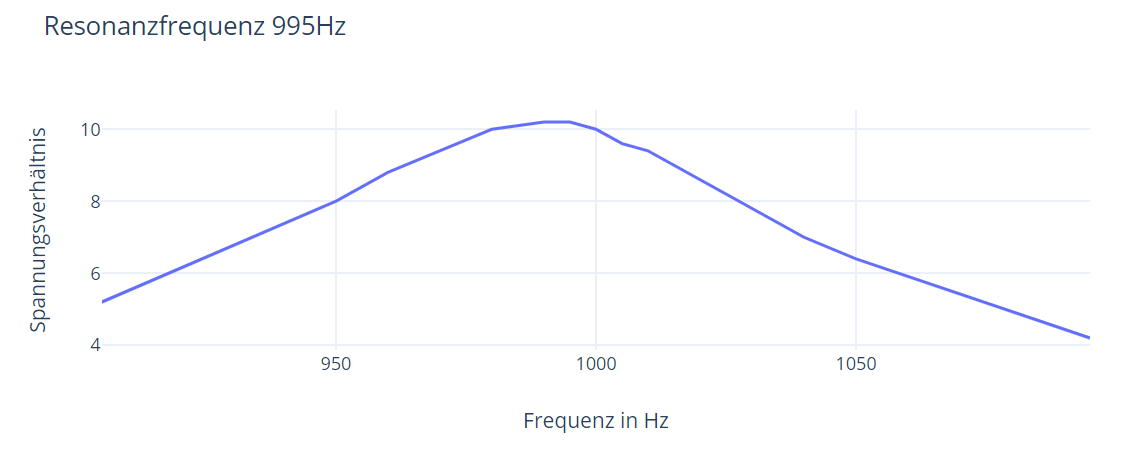
\includegraphics[scale=0.75]{../assets/images/ETP3/Fre995Plot2.PNG}
    \caption{Darstellung des Spannungsverhältnisses in Abhängigkeit der Frequenz ($f_r = 995Hz$)}
  \end{center}
\end{figure}

Wir erkennen anhand der Messwerte eine kleine Verschiebung des erwarteten Werts der Resonanzfrequenz. Für sowohl 500Hz als auch für 10kHz
ergibt sich eine neue Resonanzfrequenz von 495Hz bzw. 995Hz, ein Unterschied von $\Delta f = -5Hz$. Diese Erkenntnisse lassen sich zum einen
mit dem Innenwiderstand $R_i = 50\Omega$ und den Leiterwiderständen der verwendeten Messleitungen erklären, die eine Dämpfung in das System integrieren.
Aus diesem Grund gleichen wir diesen Umstand im nächsten Versuch mit einem Operationsverstärker-Impedanzwandler aus. Auf den Abbildungen wird der Effekt auch
optisch sehr deutlich.
\newpage

\subsubsection{Ermittlung der Güte und der Bandbreite}

Wir berechnen die Bandbreite $\Delta$f über die Formel aus der Vorbereitung, wobei wir hier
Q über $\frac{\hat{u}_C}{\hat{u}_{gen}}$ berechnen.

\begin{table}[h]
  \begin{center}
    \begin{tabular}{|c|c|c|}
      \hline
      Resonanzfrequenz & 495Hz   & 995Hz  \\
      \hline
      Q                & 5,12    & 10,2   \\
      \hline
      $\Delta$f        & 96,6797 & 97,549 \\
      \hline
    \end{tabular}
    \caption{Aus den Messwerten berechnete Güte und Bandbreite}
    \label{tab:eMGB}
  \end{center}
\end{table}

Wir erkennen, dass die Güte und die Bandbreite der Versuch ermittelten Resonanzfrequenz den vorrausberechneten Resonanzfrequenzen
stark ähneln, da wir auch nur eine leichte Abweichung von der angenommenen Resonanzfrequenz erreicht haben.

\newpage

\subsection{Versuch 2}

\begin{task}
  IIm nächsten Abschnitt soll nun mithilfe eines Operationsverstärker-Impedanzwandlers
  der Innenwiderstand des Generators abgekoppelt werden. Um keine Verzerrungen bei der Erfassung
  des Signals zu bekommen, ist es hilfreich die Generatorspannung $\hat{u}_{gen}$ geringer zu wählen.
  Wir haben uns für $\hat{u}_{gen} = 0.3V_{pp}$ entschieden
\end{task}
\begin{figure}[h]
  \begin{center}
    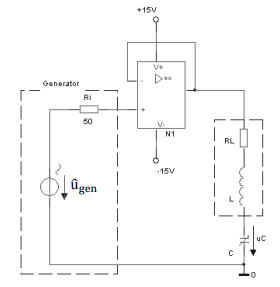
\includegraphics{../assets/images/ETP3/Versuch2Schaltplan.PNG}
    \caption{Schaltplan für den zweiten Versuch mit Operationsverstärker-Impedanzwandler}
  \end{center}
\end{figure}
\subsubsection{Bestimmung von $\frac{\hat{u}_C}{\hat{u}_{gen}}$}

Da nun nicht mehr $\frac{\hat{u}_C}{\hat{u}_{gen}} = \frac{\hat{u}_C}{1V}$ gilt, geben wir hier $\hat{u}_C$ getrennt davon nocheinmal an. 

\begin{table}[h]
  \begin{center}

    \begin{tabular}{|c|c|c|c|c|}
      \hline
                 & \multicolumn{2}{c|}{$f_r = 500Hz, C = 1,01\mu F$} & \multicolumn{2}{c|}{$f_r = 1kHz, C= 253,3 nF$}                                                   \\
      \hline
      $\Delta f$ & $\hat{u}_C$                                       & $\frac{\hat{u}_C}{\hat{u}_{gen}}$              & $\hat{u}_C$ & $\frac{\hat{u}_C}{\hat{u}_{gen}}$ \\
      \hline
      -95        & 0,56V                                             & 1,86                                           & 0,96V       & 3,2                               \\
      \hline
      -50        & 0,88V                                             & 2,93                                           & 1,6V        & 5,3                               \\
      \hline
      -40        & 1,04V                                             & 3,46                                           & 2,08V       & 6,93                              \\
      \hline
      -20        & 1,68V                                             & 5,6                                            & 4,72V       & 15,73                             \\
      \hline
      -10        & 2,96V                                             & 9,86                                           & 7,84V       & 26,13                             \\
      \hline
      -5         & 4V                                                & 13,3                                           & 7,68V       & 25,6                              \\
      \hline
      0          & 4,24V                                             & 14,13                                          & 6,24V       & 20,8                              \\
      \hline
      5          & 3,6V                                              & 12                                             & 4,88V       & 16,26                             \\
      \hline
      10         & 2,8V                                              & 9,3                                            & 3,84V       & 12,8                              \\
      \hline
      20         & 1,6V                                              & 5,3                                            & 2,56V       & 8,53                              \\
      \hline
      40         & 1,04V                                             & 3,46                                           & 1,52V       & 5,06                              \\
      \hline
      50         & 0,64V                                             & 2,13                                           & 1,2V        & 4                                 \\
      \hline
      95         & 0,48V                                             & 1,6                                            & 0,64V       & 2,13                              \\
      \hline
    \end{tabular}
    \caption{Messwerte für Versuch 2}
    \label{tab:MV2}
  \end{center}
\end{table}

\subsubsection{Graphische Darstellung}
\begin{figure}[h]
  \begin{center}
    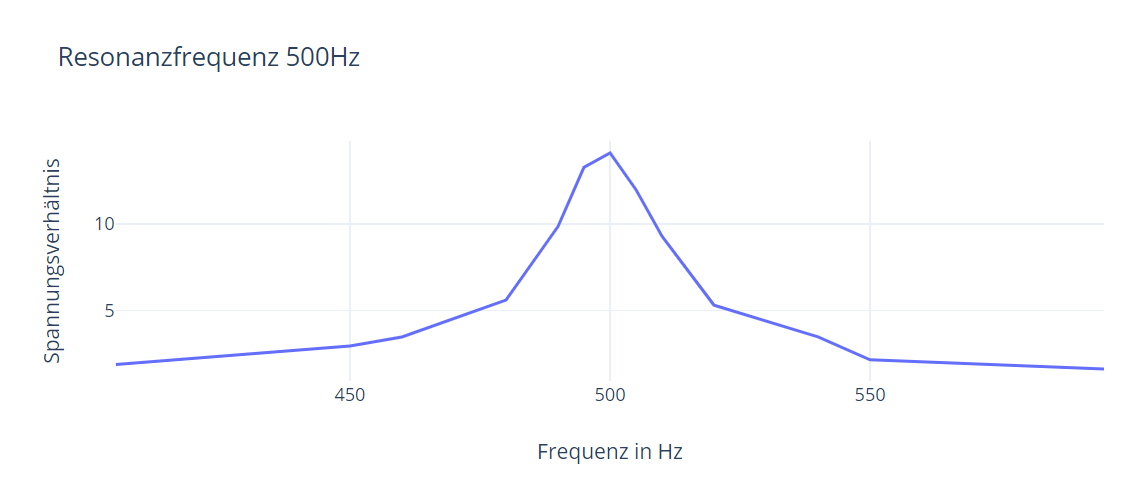
\includegraphics[scale=0.75]{../assets/images/ETP3/Fre500Plot3.PNG}
    \caption{Spannungsverhältnis abgetragen gegen die Frequenz mit Impedanzwandler ($f_r = 500Hz$)}
  \end{center}
\end{figure}

\begin{figure}[h]
  \begin{center}
    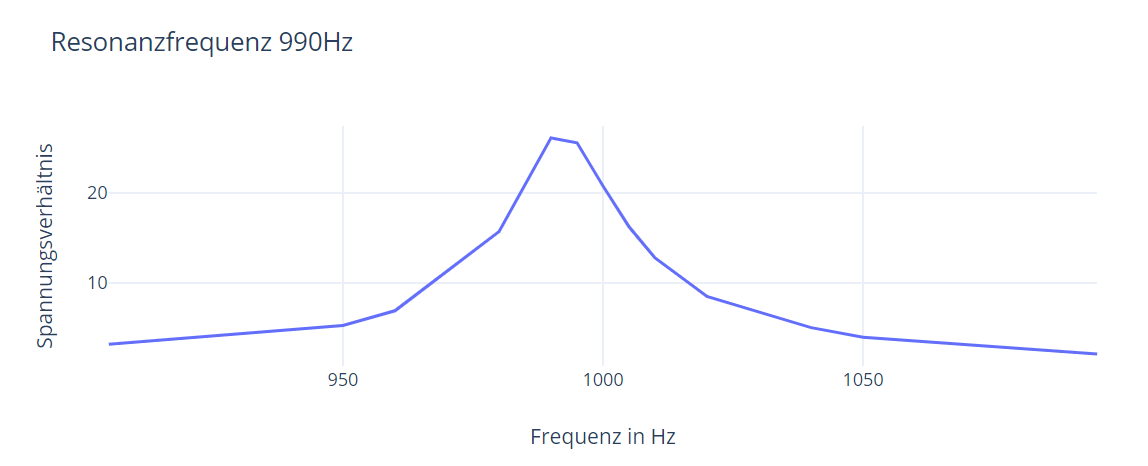
\includegraphics[scale=0.75]{../assets/images/ETP3/Fre990Plot5.PNG}
    \caption{Spannungsverhältnis abgetragen gegen die Frequenz mit Impedanzwandler ($f_r = 990Hz$)}
  \end{center}
\end{figure}
Es ist eine deutliche Erhöhung der Steigung um die Resonanzfrequenz herum erkennbar, die aus der jetzt ungedämpften Schwingung
der Generatorspannung und der Kondensatorspannung hervorgeht. Wir erkennen zudem eine kleine Verschiebung der Resonanzfrequenz im Gegensatz zum ersten Versuch,
wobei wir in der Messung um 500Hz eine Verbesserung auf genau 500Hz erzielen. Bei der Messung um 1000Hz driften wir jedoch weiter vom vorrausgesagtem Wert ab auf 990Hz.

\newpage

\subsubsection{Berechnung der Güte und der Bandbreite}

\begin{table}[h!]
  \begin{center}
    \begin{tabular}{|c|c|c|}
      \hline
      Resonanzfrequenz & 500 & 990 \\
      \hline
      Q                &  14,13   &  26,13   \\
      \hline
      $\Delta$f        &  35,3857   &  37,8874   \\
      \hline
    \end{tabular}
    \caption{Aus den Messwerten berechnete Güte und Bandbreite}
    \label{tab:zMGB}
  \end{center}
\end{table}



\subsection{Vergleich}

Es wird ein sehr deutliche Bild erkenntlich, indem der Ausgleich des dämpfenden Innenwiderstands der
Spannungsquelle ein deutlicheres Ergebnis im Bezug auf die Resonanzfrequenz und den entsprechenden Spannungsverhältnissen zulässt.
Es ist jedoch zu bemerken, dass ein solcher Operationsverstärker das Äquivalent


\subsection{Versuch mit höheren Resonanzfrequenzen}

\begin{table}[h]

  \begin{center}

    \begin{tabular}{|c|c|c|c|c|}
      \hline $\mathrm{f}$       & $\mathrm{C}$        & $\hat{u}_{g e n}$ & $\hat{u}_C$       & $\mathrm{Q}$ \\
      \hline $5 \mathrm{kH} z$  & $10,13 \mathrm{nF}$ & $300 \mathrm{mV}$ & $5,00 \mathrm{V}$ &              \\
      \hline $10 \mathrm{kH} z$ & $2,53 \mathrm{nF}$  & $300 \mathrm{mV}$ & $2,2 \mathrm{V}$  &              \\
      \hline
    \end{tabular}
    \caption{Ergebnis aus der Testreihe mit höheren Frequenzen}
    \label{tab:lCUQ}
  \end{center}
\end{table}
$$Q=\frac{1}{R} \cdot \sqrt{\frac{L}{C}} \Leftrightarrow R=\frac{1}{Q} \cdot \sqrt{\frac{L}{C}}$$
\begin{equation*}
  \text { Bei } f=5 k H z: \quad R=\frac{1}{24,1} \cdot \sqrt{\frac{100 m H}{10,13 n F}}=130,37 \Omega
\end{equation*}
\begin{equation*}
  \text { Bei } f=10 \mathrm{kHz}: \quad R=\frac{1}{19,28} \cdot \sqrt{\frac{100 \mathrm{mH}}{2,53 \mathrm{nF}}}=326,1 \Omega
\end{equation*}

\newpage
\section{Resonanz - Schaltverhalten}
\begin{task}
  IIn diesem Versuch wird wieder die Schaltung aus 1.1 aufgebaut. Für die Messungen wird zwischen dem Generator und der Spule/C-Dekade eine Präzisions-Widerstandsdekade verschaltet.
  Die Kreisresonanz wird mit der C-Dekade auf f = 1kHz eingestellt. An die Schaltung wird eine symmetrische Rechteckspannung mit einer Frequenz f = 50Hz, Tastverhältnis a = 0,5 und einem Scheitelwert von $\hat{u}_{gen} = 1,0 V$ angelegt.
  Der zeitliche Verlauf der Spannung am Kondensator wird mittels Oszilloskop dargestellt
\end{task}

\begin{devlist}
  T
  \begin{itemize}
    \item Oszilloskop: Tektronix MDO3012
    \item Kapazitätsdekade Time Electronics Model 1071 CapBox
    \item Funktionsgenerator: Keysight 33210A
    \item Multimeter: MetraHit X-TRA Multimeter
  \end{itemize}
\end{devlist}

\subsection{Serienschwingkreis mit Dämpfung}

Abbildung gedämpfter Schwingkreis\\\\

Messwerte:
\begin{table}[h]
  \begin{center}

    \begin{tabular}{|c|c|c|}
      \hline
      $T_d$ & $y_i$ & $y_{i+1}$ \\
      \hline
      1ms   & 2,64V & 2,160V    \\
      \hline
    \end{tabular}
  \end{center}
\end{table}
Berechnung des Dämpfungsmaß:
\begin{align*}
  \delta   & = \frac{1}{T_d} \cdot \ln \left(\frac{Y_i}{Y_{i+1}}\right) = 200,67      \\
  \omega   & = 2\pi \cdot f = 2\pi \cdot \frac{1}{T_d} = 6,283kHz                     \\
  \omega_r & = \frac{1}{\sqrt{LC}} = \frac{1}{\sqrt{100mH \cdot 253,3nF}} = 6,283 kHz
\end{align*}


\subsection{Aperiodischer Grenzfall}

Abbildung Aperiodischer Grenzfall

Wert liegt circa bei 1,0774kOhm

\end{document}